\documentclass[11pt,a4paper]{article}

% ---------------------------------------------------------------- packages
\usepackage[T1]{fontenc}
\usepackage{lmodern}
\usepackage{microtype}
\usepackage[margin=3.1cm]{geometry}

\usepackage{amsmath,amssymb,amsthm}
\usepackage{mathtools}
\usepackage{booktabs}
\usepackage{array}
\usepackage{caption}
\usepackage[ruled,vlined,linesnumbered]{algorithm2e}
\usepackage{tikz}
\usetikzlibrary{arrows.meta,positioning,calc,decorations.pathreplacing}
\usepackage{listings}
\usepackage[hidelinks]{hyperref}

\usepackage[backend=biber,style=alphabetic,maxbibnames=6]{biblatex}

% ---------------------------------------------------------------- theorems
\theoremstyle{plain}
\newtheorem{theorem}{Theorem}[section]

% ---------------------------------------------------------------- notation
\newcommand{\F}{\mathbb{F}_2}                  % the two-element field
\newcommand{\W}[1]{\mathsf{W}_{#1}}            % wiring by truth-table index
\newcommand{\wir}{w}                           % a generic wiring
\newcommand{\cxor}{\mathrm{cxor}}
\newcommand{\tape}{x}
\newcommand{\tab}{s}
\newcommand{\out}{r}
\newcommand{\addrset}{A}
\newcommand{\addr}[1]{a_{#1}}                  % the address in force at step #1
\newcommand{\cell}[1]{\tab[#1]}                % one bit of storage
\newcommand{\code}[1]{\texttt{#1}}
\newcommand{\bstr}[1]{\text{\texttt{#1}}}

% ---------------------------------------------------------------- listings
\lstset{basicstyle=\ttfamily\small, keywordstyle=\bfseries,
        commentstyle=\itshape, columns=fullflexible, frame=leftline,
        framesep=8pt, xleftmargin=10pt, showstringspaces=false, language=Python}

\addbibresource{paper.bib}

\title{%
  \texorpdfstring{{\Huge\bfseries$\mathbf{cxor}$}}{cxor}\\[6pt]
  {\large A One-Bit Context Transform over \texorpdfstring{$\F$}{F2}}\\[-5pt]
  {\large and Its Sixteen Update Rules}}
\author{Yauhen Yakimovich\\
        \small\href{mailto:yauhen.yakimovich.mail@gmail.com}{yauhen.yakimovich.mail@gmail.com}}
\date{\today}

\begin{document}
\maketitle

\begin{abstract}
Context Transformation Algorithms (CTA) originated as a broader family of context-addressed
transforms.  This paper isolates one binary member, called $\cxor$ (CTA-XOR), in which every
$m$-bit context addresses a single bit of state and the source symbol is combined with that state
by addition in $\F$.  Reading the state as a hard next-bit prediction makes the emitted bit a
prediction residual: zero denotes a correct prediction and one an error.  The historically
implemented update $\W5(s,x)=x$ replaces the prediction with the observation, so a context
predicts that its next successor will equal its most recently observed successor.

$\cxor$ is not itself a compressor: it is length preserving and bijective.  Its possible use is
to expose contextual predictability as a zero-rich residual for a subsequent coder.  We prove
that sequential decoding follows from causality and does not depend on the particular update
rule.  Under the deliberately narrow one-bit $\cxor$ assumptions, an update is an arbitrary
Boolean function of the old state and current symbol, giving exactly sixteen wirings.  Algebraic
normal form separates eight affine rules, whose per-context behaviour reduces to the three
operators $1$, $1+T$, and $(1+T)^{-1}$, from eight data-dependent rules.  The same analysis yields
four adaptation horizons.  $\W5$ realises contextual differencing and forgets an old prediction
after one observation; $\W6$ realises running parity and retains its old state indefinitely.  At
context order zero these are the two directions of binary Gray coding.
\end{abstract}

\section{From context modelling to \texorpdfstring{$\cxor$}{cxor}}\label{sec:intro}

Statistical compression begins by assigning probabilities to the next symbol.  In a binary
order-$m$ context model, the $m$ most recent source bits select one of $2^m$ contexts, and the
model records what has followed that context in the past.  Prediction by partial matching (PPM),
for example, keeps symbol counts at several context orders and uses an escape mechanism when a
long context is uninformative \cite{bell1990text}.  A probability model and an entropy coder then
turn accurate probability estimates into a short representation.

Context Transformation Algorithms (CTA) denotes the broader idea of associating state with
contexts and using it to transform a source.  This paper studies one deliberately restricted
binary member, which we call $\cxor$ (CTA-XOR):
\[
  {\small
    \text{Context Transformation Algorithms (CTA)}
    \supset
    \text{$\cxor$ over $\F$}
    \supset
    \text{the historical $\W5$ instance}.}
\]

$\cxor$ can be reached from context modelling by asking how little of the architecture can
remain.  Give each context exactly one bit of state and interpret that bit as a hard prediction
$\hat x$ of the next source bit.  When the actual bit $x$ arrives, emit
\begin{equation}\label{eq:residual-intro}
  r=x\mathbin{\oplus}\hat x .
\end{equation}
Then $r=0$ means that the context predicted correctly, while $r=1$ means a prediction error.  The
result is simultaneously a context-indexed predictor and a residual transform.

The historically implemented update is as small as the state.  After observing $x$, store $x$ in
the cell for the current context:
\begin{equation}\label{eq:w5-intro}
  \W5(s,x)=x .
\end{equation}
Thus the next time the same context occurs, $\W5$ predicts that it will have the same successor as
last time.  It has one bit per context, immediate adaptation, and no counts, probabilities,
confidence, escape, or backoff.  This predictor interpretation is not an analogy added after the
fact: it is exactly the read--compare--update sequence in the earlier $\cxor$ implementation.

The residual can be more skewed than the source.  With context order $m=4$, the example shipped
with the reference $\W5$ program is
\begin{center}
\begin{tabular}{@{}r@{\ }l@{}}
input:       & \bstr{101001110111011111011111111111110}\\
$\cxor_{\W5}$: & \bstr{101001110111000011100001000000001}\\
inverse:     & \bstr{101001110111011111011111111111110}.
\end{tabular}
\end{center}
The input has $7$ zeros and $26$ ones; its image has $20$ zeros and $13$ ones.  The useful
observation is zero enrichment: repeated contextual regularity has become a concentration of
prediction successes.  The example is not evidence of compression, and no compression result is
claimed here.  $\cxor$ emits exactly one bit for every input bit and can be inverted exactly.

The paper first defines this predictor and its decoder, then makes precise which regularities
$\W5$ can expose and why their exposure is separate from both invertibility and compression.
Only after that do we vary the learning rule.  Within the one-bit $\cxor$ architecture, if a cell
may be updated using only its old value $s$ and the observed bit $x$, the update is a Boolean function
\[
  w:\mathbb F_2^2\longrightarrow\mathbb F_2,
\]
and there are exactly $2^{2^2}=16$ possibilities.  This finite design space classifies the narrow
$\cxor$ model, not the CTA family.

The construction studied here originated in earlier unpublished work by the author on the
broader CTA family.  That work existed in manuscript and implementation form, but the binary XOR
construction was never published as a separate, self-contained treatment.  The present paper
extracts that operation from the broader line of work, formalises it independently, and calls it
$\cxor$.

The analysis makes four contributions.
\begin{enumerate}
  \item It identifies the historical $\W5$ implementation as a last-observation context predictor
        followed by an exclusive-or residual.
  \item It proves that causal prediction makes every one of the sixteen transforms sequentially
        invertible; reversibility comes from the predictor/residual construction, not from a
        special feature of $\W5$.
  \item It classifies the rules by algebraic normal form.  The eight affine rules admit a compact
        per-context operator description and realise only $1$, $1+T$, or $(1+T)^{-1}$; the other
        eight have data-dependent state retention.
  \item It interprets the resulting memory horizons as adaptation behaviour.  $\W5$ replaces an
        old belief after one observation, whereas $\W6(s,x)=s\oplus x$ preserves old state.
\end{enumerate}

Three notions will remain separate throughout.  \emph{Prediction performance} is a property of a
rule, a context order, and a particular source; it can be measured by the residual zeros.
\emph{Invertibility} is structural and holds even when every prediction is poor.
\emph{Compression} requires an additional model and coder.  Confusing any two of these obscures
what $\cxor$ does.

\section{The \texorpdfstring{$\cxor$}{cxor} architecture}\label{sec:cta}

Let $\F=\{0,1\}$, with addition interpreted as exclusive-or.  Fix a context order $m\ge0$.
The context set is $A=\F^m$, and a table $s:A\to\F$ contains one bit for every context.  Before
the input starts, the table has a known initial value $s_0$ and the context window has a known
prefix $\pi\in\F^m$.  The reference $\W5$ program uses zeros for both.

For an input $x=x_0x_1\dots x_{n-1}$, the address $a_k$ at position $k$ is the length-$m$ suffix
of $\pi x_0\dots x_{k-1}$.  In particular, $a_k$ contains only source symbols \emph{strictly
before} $x_k$.  At a step, write $u=s[a_k]$ for the state read from the addressed cell.  The
general datapath is
\begin{equation}\label{eq:machine-step}
  r_k=x_k+u,
  \qquad
  s[a_k]\leftarrow w(u,x_k),
\end{equation}
where $w$ is a one-bit update rule.  The historical instance uses $w=\W5$, so the second
assignment is simply $s[a_k]\leftarrow x_k$.

\begin{figure}[ht]
  \centering
  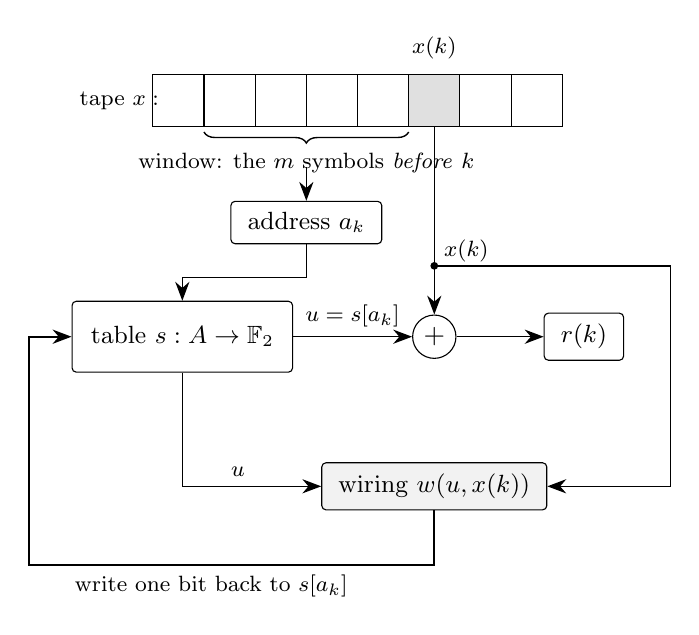
\begin{tikzpicture}[
    >={Stealth[length=2.4mm]},
    box/.style={draw, rounded corners=1.5pt, inner xsep=6pt, inner ysep=4pt, font=\small},
    cell/.style={draw, minimum size=6.5mm, inner sep=0pt, font=\footnotesize},
    xorg/.style={draw, circle, minimum size=5.5mm, inner sep=0pt},
    lbl/.style={font=\footnotesize},
    wire/.style={line width=0.5pt},
  ]
  % ---------------- tape
  \node[cell] at (2.35,4.3) {};
  \foreach \p in {3.0,3.65,4.3,4.95} { \node[cell] at (\p,4.3) {}; }
  \node[cell, fill=black!12] (ck) at (5.6,4.3) {};
  \node[cell] at (6.25,4.3) {};
  \node[cell] at (6.9,4.3) {};
  \node[lbl] at (1.6,4.3) {tape $\tape:$};
  \node[lbl, above=2pt of ck] {$\tape(k)$};
  \draw[decorate, decoration={brace, amplitude=4pt, mirror}, wire]
       (2.675,3.9) -- (5.275,3.9)
       node[midway, below=4pt, lbl] {window: the $m$ symbols \emph{before} $k$};

  % ---------------- address
  \node[box] (adr) at (3.975,2.75) {address $\addr{k}$};
  \draw[->,wire] (3.975,3.45) -- (adr.north);

  % ---------------- table
  \node[box, minimum width=2.8cm, minimum height=9mm] (tab) at (2.4,1.3)
       {table $\tab:\addrset\to\F$};
  \draw[->,wire] (adr.south) -- (3.975,2.05) -- (2.4,2.05) -- (tab.north);

  % ---------------- emitter
  \node[xorg] (xr) at (5.6,1.3) {$+$};
  \draw[->,wire] (tab.east) -- node[above, lbl] {$u=\cell{\addr{k}}$} (xr.west);
  \draw[->,wire] (ck.south) -- node[right, lbl, pos=0.66] {$\tape(k)$} (xr.north);
  \node[box] (out) at (7.5,1.3) {$\out(k)$};
  \draw[->,wire] (xr.east) -- (out.west);

  % ---------------- wiring
  \node[box, minimum width=2.4cm, fill=black!5] (w) at (5.6,-0.6) {wiring $\wir(u,\tape(k))$};
  \draw[->,wire] (tab.south) -- (2.4,-0.6) -- node[above,lbl,pos=0.4] {$u$} (w.west);
  \fill (5.6,2.2) circle (1.4pt);
  \draw[->,wire] (5.6,2.2) -- (8.6,2.2) -- (8.6,-0.6) -- (w.east);

  % ---------------- write-back
  \draw[->,wire, line width=0.8pt]
       (w.south) -- (5.6,-1.6) -- node[below, lbl, pos=0.55] {write one bit back to $\cell{\addr{k}}$}
       (0.45,-1.6) -- (0.45,1.3) -- (tab.west);
\end{tikzpicture}

  \caption{One $\cxor$ step.  The preceding $m$ source symbols address a one-bit prediction; the
  exclusive-or emits a residual; and the update rule writes the addressed cell.  In the
  historical $\W5$ implementation the shaded update is $\W5(u,x)=x$.}
  \label{fig:cxor-datapath}
\end{figure}

\begin{algorithm}[ht]
\caption{$\cxor_w$; choose $w=\W5$ for the historical instance}\label{alg:cxor}
\DontPrintSemicolon
$c\leftarrow\pi$; $s\leftarrow s_0$\;
\For{$k\leftarrow0$ \KwTo $n-1$}{
  $a\leftarrow c$; $u\leftarrow s[a]$\;
  $r_k\leftarrow x_k+u$\;
  $s[a]\leftarrow w(u,x_k)$\;
  $c\leftarrow\operatorname{suffix}_m(c x_k)$\;
}
\Return $r$
\end{algorithm}

The ordering matters.  The lookup precedes the window shift, so the prediction is causal.  The
current symbol is used to update the prediction only after its residual has been emitted.

\subsection{Why the reference code is exactly \texorpdfstring{$\W5$}{W5}}

The reference implementation expresses its update conditionally:
\begin{lstlisting}
diff = state != x
out_bits.append(diff)
if diff:
    lookup[index] = x
\end{lstlisting}
For bits, \code{state != x} is $s[a_k]\oplus x_k$, so \code{diff} is precisely the residual
$r_k$.  When \code{diff} is true, the code stores $x_k$.  When it is false, the assignment is
unnecessary because $s[a_k]=x_k$ already.  Consequently the conditional is equivalent to the
unconditional update
\[
  s[a_k]\leftarrow x_k,
\]
which is $\W5$.  Operationally, the program reads the prediction, reports whether it was wrong,
and makes the new prediction equal to the observation.

\subsection{A small trace}

Take $m=2$, a zero prefix and table, and the periodic input $x=\bstr{010101010}$.  The first
occurrences of contexts $\bstr{01}$ and $\bstr{10}$ establish their successors.  Thereafter the
same associations repeat, so their residuals are zero.

\begin{table}[ht]
\centering\small
\begin{tabular}{@{}rccccc@{}}
\toprule
$k$ & context $a_k$ & source $x_k$ & prediction $u$ & residual $r_k$ & new prediction\\
\midrule
0 & \bstr{00} & 0 & 0 & 0 & 0\\
1 & \bstr{00} & 1 & 0 & 1 & 1\\
2 & \bstr{01} & 0 & 0 & 0 & 0\\
3 & \bstr{10} & 1 & 0 & 1 & 1\\
4 & \bstr{01} & 0 & 0 & 0 & 0\\
5 & \bstr{10} & 1 & 1 & 0 & 1\\
6 & \bstr{01} & 0 & 0 & 0 & 0\\
7 & \bstr{10} & 1 & 1 & 0 & 1\\
8 & \bstr{01} & 0 & 0 & 0 & 0\\
\bottomrule
\end{tabular}
\caption{$\W5$ on a two-bit context.  The output is $\bstr{010100000}$.  Each zero is a correct
hard prediction, including initial predictions from the zero table.}
\label{tab:small-w5-trace}
\end{table}

The trace also shows why periodicity is only a special case of the mechanism.  The machine does
not search for a period; it independently remembers that $\bstr{01}$ was followed by $0$ and
$\bstr{10}$ by $1$.

\subsection{Sequential decoder}

The residual loses no information.  A decoder starts with the same prefix, table, and update
rule.  Suppose it has already recovered $x_0,\dots,x_{k-1}$.  Those bits determine $a_k$, and
replaying the same updates determines the encoder's current $u=s[a_k]$.  Hence
\begin{equation}\label{eq:decode-short}
  x_k=r_k+u.
\end{equation}
The decoder then applies $s[a_k]\leftarrow w(u,x_k)$ and advances the window with the recovered
symbol.  This proves the following general fact.

\begin{theorem}[Causal residuals are invertible]\label{thm:causal-inverse}
For every $m$, initial table $s_0$, prefix $\pi$, deterministic update rule $w$, and length $n$,
Algorithm~\ref{alg:cxor} is a bijection $\F^n\to\F^n$.
\end{theorem}

\begin{proof}
Equation~\eqref{eq:decode-short} recovers the input sequentially.  Induction on $k$ shows that
encoder and decoder have identical windows and tables before every step, so the recovery is
unique.  The resulting inverse maps the finite set $\F^n$ onto itself.
\end{proof}

The proof does not invert $w$ and uses no special property of $\W5$.  It inverts the exclusive-or
emitter using a prediction reproducible from the already decoded prefix.  This is the same causal
principle used by predictive lossless codes with much richer predictors.

If the window were shifted before lookup, so that $x_k$ participated in its own address, the
decoder would in general need $x_k$ to discover the prediction required to recover $x_k$.
Collisions then occur for ordinary nonzero tables.  The lagging, source-driven address in
Algorithm~\ref{alg:cxor} is therefore part of the transform, not a cosmetic indexing convention.

\section{The \texorpdfstring{$\W5$}{W5} instance as a predictive transform}\label{sec:predictive}

The one-bit state has a direct operational meaning under $\W5$.  Fix a context $a$, and list the
positions at which it occurs as
\[
  k_0<k_1<k_2<\cdots .
\]
Let $y_j=x_{k_j}$ be the symbol that follows that occurrence of $a$.  If the initial cell is
$q_a$, $\cxor_{\W5}$ emits
\begin{equation}\label{eq:w5-per-context}
  r_{k_0}=y_0+q_a,
  \qquad
  r_{k_j}=y_j+y_{j-1}\quad(j\ge1).
\end{equation}
The first visit is predicted from the initial table.  Every later visit compares the current
successor with the successor observed on the preceding visit to the same context.  Thus $\W5$ is
contextual differencing: after the first visit, a zero says exactly that the association
$a\mapsto y$ has repeated.

This gives a more accurate description than saying that $\W5$ detects periodic substrings.
$\W5$ suppresses repeated context-to-successor associations.  Periodic and locally repetitive
sources are important special cases: once an $m$-bit context recurs with a stable successor,
subsequent visits to that context emit zero.  But periodicity is neither necessary nor sufficient
as a source-wide description.  Different contexts may recur at irregular intervals, and a
repeated context whose successor alternates will produce errors rather than zeros.

\subsection{What determines zero enrichment}

The residual depends jointly on the source and the model order.
\begin{itemize}
  \item \emph{Context order.}  A small $m$ merges histories that may have different successors;
        a large $m$ separates them but creates more cells to learn.
  \item \emph{Input length and recurrence.}  There are $2^m$ possible contexts.  On a short input,
        many are never revisited, so their one-bit memories cannot contribute a learned
        prediction.  A context seen only once is predicted solely from its initial cell.
  \item \emph{Successor stability.}  Recurrence helps only when repeated occurrences tend to have
        the same following bit.  Equation~\eqref{eq:w5-per-context} makes this dependence exact.
  \item \emph{Initialisation.}  The initial table affects the first visit to each context.  The
        zero table used by the reference implementation initially predicts zero everywhere;
        $\W5$ overwrites that choice after one observation.
\end{itemize}

The example in the introduction illustrates these conditions rather than proving a general
gain.  Its 33 symbols are long enough to revisit several four-bit contexts, and enough of those
contexts repeat their successor that the residual contains 20 zeros instead of 7.  On another
source, or with another $m$, $\W5$ may leave the marginal balance unchanged or make it less
favourable.  Prediction performance is therefore empirical even though the transform is exact.

\subsection{Why this is not compression}

$\cxor_w$ maps $n$ input bits to $n$ residual bits, and Theorem~\ref{thm:causal-inverse} says that
it permutes the $2^n$ possible strings for every wiring.  It does not reduce length or information
entropy by itself.
The intended architecture, if the residual is useful, is
\[
  x
  \longrightarrow
  \text{$\cxor_{\W5}$ residual}
  \longrightarrow
  \text{statistical model and entropy coder}.
\]
A downstream coder might exploit a residual with a strong zero bias, long zero runs, or other
simple structure more easily than it exploits the original context dependence.  Whether it
actually does so depends on that coder and on the source; it is an experimental question not
answered by the algebra in this paper.

The role is analogous in spirit to other reversible preprocessing transforms.  The
Burrows--Wheeler transform, for example, is valuable because it presents existing dependence in
a form suitable for simple back ends, not because the permutation itself shortens the data
\cite{burrows1994block}.  $\cxor_{\W5}$ uses a causal predictor rather than block sorting, so the analogy
should not be taken further.

Zero frequency, invertibility, and compressed size therefore answer different questions.  The
first measures hard-prediction success for a specific run.  The second is guaranteed by causal
decoding.  The third can be known only after a downstream representation has been specified.

\section{The sixteen one-bit update rules}\label{sec:wirings}

The one-bit $\cxor$ model fixes the address calculation and residual emitter, leaving only the
cell update to vary.  If the update can inspect only the old state $s$ and current source bit
$x$, it is a function $w:\F^2\to\F$.  Four input pairs must each be assigned one output bit, so
there are
\[
  2^{|\F^2|}=2^4=16
\]
rules.  This is the complete update space under the one-cell, one-bit $\cxor$ restriction.

We name a rule by reading
\[
  w(0,0)\,w(0,1)\,w(1,0)\,w(1,1)
\]
as a four-bit binary integer, most significant bit first.  Thus the projection $w(s,x)=x$ has
truth table $0101$ and is $\W5$, while exclusive-or $w(s,x)=s+x$ has table $0110$ and is
$\W6$.

Every two-variable Boolean function has a unique algebraic normal form (ANF)
\begin{equation}\label{eq:anf-new}
  w(s,x)=d_0+d_1s+d_2x+d_3sx,
  \qquad d_i\in\F .
\end{equation}
Indeed, evaluating at $(0,0),(1,0),(0,1),(1,1)$ successively determines
\begin{equation}\label{eq:anf-coeff}
  d_0=w(0,0),\quad d_1=w(1,0)+d_0,\quad d_2=w(0,1)+d_0,
  \quad d_3=w(1,1)+d_0+d_1+d_2.
\end{equation}
This standard representation \cite{carlet2010boolean} exposes the classification needed below:
$d_3=0$ gives an \emph{affine} update, while $d_3=1$ couples the retained state to the observed
data.  In the language of Post's classification, the eight rules with $d_3=0$ constitute the
affine class \cite{post1941}; no further lattice machinery is needed here.

\begin{table}[ht]
\centering\small
\begin{tabular}{@{}clll@{\qquad}clll@{}}
\toprule
rule & truth & ANF & kind & rule & truth & ANF & kind\\
\midrule
$\W0$  & \bstr{0000} & $0$                 & affine & $\W8$  & \bstr{1000} & $1+s+x+sx$ & nonlinear\\
$\W1$  & \bstr{0001} & $sx$                & nonlinear & $\W9$  & \bstr{1001} & $1+s+x$ & affine\\
$\W2$  & \bstr{0010} & $s+sx$              & nonlinear & $\W{10}$ & \bstr{1010} & $1+x$ & affine\\
$\W3$  & \bstr{0011} & $s$                 & affine & $\W{11}$ & \bstr{1011} & $1+x+sx$ & nonlinear\\
$\W4$  & \bstr{0100} & $x+sx$              & nonlinear & $\W{12}$ & \bstr{1100} & $1+s$ & affine\\
$\W5$  & \bstr{0101} & $x$                 & affine & $\W{13}$ & \bstr{1101} & $1+s+sx$ & nonlinear\\
$\W6$  & \bstr{0110} & $s+x$               & affine & $\W{14}$ & \bstr{1110} & $1+sx$ & nonlinear\\
$\W7$  & \bstr{0111} & $s+x+sx$            & nonlinear & $\W{15}$ & \bstr{1111} & $1$ & affine\\
\bottomrule
\end{tabular}
\caption{The complete update-rule space.  Addition and multiplication are in $\F$.  ``Nonlinear''
means $d_3=1$ in ANF; the resulting recurrence has data-dependent state retention.}
\label{tab:new-wirings}
\end{table}

Two rules deserve names beyond their indices:
\begin{align}
  \W5(s,x)&=x,
  &\text{last-observation update,}\label{eq:w5-rule}\\
  \W6(s,x)&=s+x,
  &\text{running-parity update.}\label{eq:w6-rule}
\end{align}
$\W5$ is the rule used by the earlier $\cxor$ implementation.  It discards the old cell after
every observation and stores the successor just seen.  $\W6$ instead writes $s+x$, which is also the emitted residual
$r$ at that step.  Along repeated visits to one context it accumulates the parity of all observed
successors.  Although the same emitter permits reading its state as a hard prediction, its update
does not learn ``what followed this context last'' and is not naturally a next-symbol predictor.
It enters because it is the algebraic counterpart of $\W5$, not because it shares $\W5$'s modelling
interpretation.

All sixteen rules use the same causal emitter and are therefore invertible by
Theorem~\ref{thm:causal-inverse}.  The classification below asks what the update changes, rather
than using invertibility to choose an update.

\section{Structure of the transform}\label{sec:structure}

The address sequence interleaves $2^m$ one-cell machines.  Once those machines are separated, the
algebra of the sixteen rules becomes transparent.

\subsection{Per-context decomposition}

Fix an input and prefix.  For a context $a$, let $k_{a,0}<k_{a,1}<\cdots$ be its visits, set
$y_{a,j}=x_{k_{a,j}}$, and let $u_{a,j}$ be cell $a$ immediately before its $j$th visit.  Directly
from Algorithm~\ref{alg:cxor},
\begin{equation}\label{eq:per-context-general}
  r_{k_{a,j}}=y_{a,j}+u_{a,j},
  \qquad
  u_{a,j+1}=w(u_{a,j},y_{a,j}).
\end{equation}
No recurrence for $a$ reads a cell belonging to another context.  The full transform is therefore
an interleaving of independent per-context recurrences; the source itself determines the
interleaving through its preceding $m$-bit windows.

This decomposition also separates two roles that can otherwise be confused.  Addressing decides
\emph{when} a state is consulted.  The wiring decides how that state evolves \emph{between visits
to the same context}.  Invertibility needs only that the address at the next step be recoverable
from the decoded prefix, while the operator and adaptation properties below belong to the
per-context recurrence.

\subsection{Affine rules and three transfer operators}

Assume first that $d_3=0$, so
\[
  w(s,x)=d_0+d_1s+d_2x.
\]
Within one context, let $T$ mean ``previous visit to this same context'': $(Tz)_0=0$ and
$(Tz)_j=z_{j-1}$ for $j\ge1$.  The recurrence
\[
  u_{j+1}=d_0+d_1u_j+d_2y_j,
  \qquad r_j=y_j+u_j
\]
gives, after collecting the terms that depend linearly on $y$,
\begin{equation}\label{eq:new-transfer}
  r
  =
  \frac{1+(d_1+d_2)T}{1+d_1T}\,y+c .
\end{equation}
Here $c$ is an additive response determined by the initial cell and $d_0$.  Division is only
compact notation: if $d_1=1$, then
\[
  (1+T)^{-1}=1+T+T^2+\cdots,
\]
and only finitely many terms contribute at any visit.  Equation~\eqref{eq:new-transfer} is the
usual linear-recurrence calculation over $\F$ \cite{golomb1967,lincostello2004}, with delay
measured in visits rather than adjacent tape positions.

Only $(d_1,d_2)$ affects the linear operator, so the eight affine wirings realise exactly three:
\begin{table}[ht]
\centering\small
\begin{tabular}{@{}cllc@{}}
\toprule
$(d_1,d_2)$ & operator & wirings & constant-free representative\\
\midrule
$(0,0)$ or $(1,0)$ & $1$ & $\W0,\W3,\W{12},\W{15}$ & $\W0,\W3$\\
$(0,1)$ & $1+T$ & $\W5,\W{10}$ & $\W5$\\
$(1,1)$ & $(1+T)^{-1}$ & $\W6,\W9$ & $\W6$\\
\bottomrule
\end{tabular}
\caption{The affine update rules collapse to three per-context operators.  Rules paired in a row
differ only by an additive response.}
\label{tab:operators-new}
\end{table}

For $\W5$, the equation $r=(1+T)y+c$ is exactly the contextual difference in
Equation~\eqref{eq:w5-per-context}.  For $\W6$, the state accumulates past symbols and the output
is their running exclusive-or, giving $(1+T)^{-1}$.  These are the only constant-free affine
rules with nonidentity operators.

When $d_3=1$, the recurrence can instead be written
\begin{equation}\label{eq:nonaffine-recurrence}
  u_{j+1}=(d_0+d_2y_j)+(d_1+y_j)u_j .
\end{equation}
The multiplier of the old state now depends on the arriving symbol.  The input-output map is in
general nonlinear in $y$, so no fixed linear transfer operator represents these eight rules.
They should be regarded as data-dependent updates, not as additional entries in
Table~\ref{tab:operators-new}.

The operator statement is per context, or equivalently conditional on a fixed address sequence.
For $m\ge2$, the partition of tape positions into contexts depends on the source, so $T$ itself
changes when the tape changes.  The three-operator result must not be misread as claiming that the
whole source-to-residual map is globally linear.

\subsection{Adaptation and memory horizon}

The ANF also says how long an old prediction can matter.  Run the same context sequence twice
with different initial cell bits, and let $\delta_j$ be the difference between the two states
before visit $j$.  Subtracting the two copies of Equation~\eqref{eq:anf-new} gives
\begin{equation}\label{eq:delta-horizon}
  \delta_{j+1}=(d_1+d_3y_j)\delta_j,
  \qquad
  \delta_j=\delta_0\prod_{i<j}(d_1+d_3y_i).
\end{equation}
Because the emitted residual contains the current state, the same $\delta_j$ measures the effect
of the old cell on the output at visit $j$.  Four adaptation regimes follow.

\begin{table}[ht]
\centering\small
\begin{tabular}{@{}clll@{}}
\toprule
$(d_1,d_3)$ & retention factor & wirings & adaptation horizon\\
\midrule
$(0,0)$ & $0$ & $\W0,\W5,\W{10},\W{15}$ & old state affects the first visit only\\
$(1,0)$ & $1$ & $\W3,\W6,\W9,\W{12}$ & old state is never forgotten\\
$(0,1)$ & $y$ & $\W1,\W4,\W{11},\W{14}$ & retained through $1$s; a $0$ erases it\\
$(1,1)$ & $1+y$ & $\W2,\W7,\W8,\W{13}$ & retained through $0$s; a $1$ erases it\\
\bottomrule
\end{tabular}
\caption{The four memory horizons.  For the nonlinear rules, retention is controlled by the
observed successor sequence within each context.}
\label{tab:adaptation-new}
\end{table}

$\W5$ is immediately forgetting in the intended predictive sense: after one visit, its state is
the new observation and contains no information about the previous belief.  This is maximal
adaptation for a one-bit hard predictor.  $\W6$ is the opposite affine extreme: changing the
initial cell changes every later state and residual in that context.  The nonlinear rules offer
conditional forgetting; whether an old state survives is decided by the observed symbol.  Thus
the affine/nonlinear split is also a split between fixed and data-dependent adaptation behaviour.

\section{W5, W6, and the Gray-code special case}\label{sec:special}

The two nontrivial affine operators describe very different state semantics.  Along one context
class with initial state $q$, Equations~\eqref{eq:w5-rule} and \eqref{eq:w6-rule} unwind to
\begin{align}
\W5:\quad
  r_0&=y_0+q,
  &r_j&=y_j+y_{j-1} &&(j\ge1),\label{eq:w5-unwind}\\
\W6:\quad
  r_j&=q+\sum_{i=0}^{j}y_i .&&&&\label{eq:w6-unwind}
\end{align}
$\W5$ asks whether the current successor differs from the last successor of this context.  Its
state is a prediction with a clear learning rule.  $\W6$ reports cumulative parity; because its
new state equals the emitted $r_j$, it feeds the residual back into the next visit.  Its state
continues to contain the initial bit and all previous successors.

\begin{figure}[ht]
  \centering
  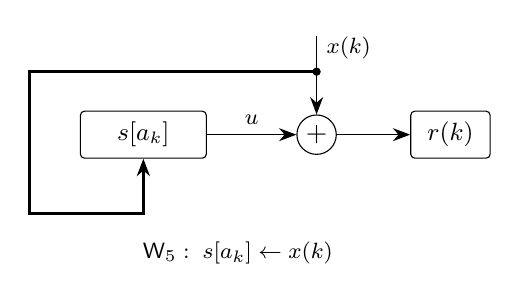
\begin{tikzpicture}[
    >={Stealth[length=2.2mm]},
    box/.style={draw, rounded corners=1.5pt, inner xsep=6pt, inner ysep=4pt, font=\small},
    xorg/.style={draw, circle, minimum size=5mm, inner sep=0pt},
    lbl/.style={font=\footnotesize},
    wire/.style={line width=0.5pt},
    fb/.style={line width=1.1pt},
  ]
  \node[box, minimum width=1.6cm] (S) at (0,0) {$\cell{\addr{k}}$};
  \node[xorg] (xr) at (2.2,0) {$+$};
  \node[box] (out) at (3.9,0) {$\out(k)$};
  \draw[->,wire] (S.east) -- node[above,lbl] {$u$} (xr.west);
  \draw[->,wire] (2.2,1.25) -- node[right,lbl,pos=0.15] {$\tape(k)$} (xr.north);
  \draw[->,wire] (xr.east) -- (out.west);
  \fill (2.2,0.8) circle (1.5pt);
  \draw[->,fb] (2.2,0.8) -- (-1.45,0.8) -- (-1.45,-1.0) -- (0,-1.0) -- (S.south);
  \node[lbl] at (1.2,-1.5) {$\W5:\; \cell{\addr{k}}\leftarrow\tape(k)$};
\end{tikzpicture}
\hspace{1.1cm}\input{fig/wiring6.tex}
  \caption{$\W5$ and $\W6$ use the same emitter.  Moving the feedback tap from before the
  exclusive-or to after it changes a last-observation predictor into a running-parity state.}
  \label{fig:w5-w6-taps}
\end{figure}

The operators $1+T$ and $(1+T)^{-1}$ are mutual inverses, but this statement has a precise scope.
If the address sequence is held fixed, applying the $\W6$ recurrence to the $\W5$ residual (or
vice versa) restores each per-context sequence.  In $\cxor$, however, addresses are generated
from the transform's current input.  Feeding a $\W5$ residual into a fresh $\W6$
encoder generally produces a different address sequence and is not the decoder of
Section~\ref{sec:cta}.  The causal decoder reconstructs source bits and reproduces the original
addresses while applying the \emph{same} update rule.  Operator duality and transform inversion
are therefore related but distinct facts.

\subsection{Order zero}

At $m=0$ there is only one context, so visits are ordinary adjacent positions and $T$ is the
usual one-step delay.  With a zero initial cell, $\W5$ gives
\begin{equation}\label{eq:gray}
  r_0=x_0,
  \qquad
  r_k=x_k+x_{k-1}\quad(k\ge1).
\end{equation}
If the bits are read most significant first as the binary representation of an integer $b$,
Equation~\eqref{eq:gray} is exactly reflected binary (Gray) encoding
\[
  g=b\mathbin{\oplus}(b\mathbin{\gg}1)
\]
\cite{gray1953}.  $\W6$ takes prefix exclusive-ors and is the corresponding Gray decoder.  This
is the simplest concrete instance of the two transfer operators.

For example, $90$ is $\bstr{01011010}$ in eight-bit binary.  $\W5$ emits
$\bstr{01110111}$, representing $119=90\oplus45$, and $\W6$ maps that word back to
$\bstr{01011010}$.  In this order-zero case the fixed-address operator duality is also an ordinary
composition of the two transforms, because there is no source-dependent address sequence to
change between passes.

For $m>0$, the delay means ``previous visit to this context'' rather than ``previous tape
position.''  At $m=1$ with zero table and prefix, $\W5$ happens to reduce to the stride-two
difference $r_k=x_k+x_{k-2}$, taking out-of-range bits as zero.  At larger orders the visit
partition is source-dependent and no fixed tape stride describes it.  Calling $\cxor$ a
generalised Gray code would therefore hide its defining feature: context-addressed prediction.
Gray coding is an elegant boundary case, not the main interpretation.

\section{From \texorpdfstring{$\cxor$}{cxor} back to statistical compression}\label{sec:ladder}

$\cxor_{\W5}$ can be read as a context model reduced to one bit, and its limitations are exactly
what that reduction removes.  A cell can say ``zero'' or ``one,'' but not ``one with probability
$0.9$.''  It cannot distinguish a prediction supported by one observation from one supported by
a thousand.  $\W5$ changes its mind after every error, has no escape when a context is new, and
cannot share evidence between related contexts.

Putting capacity back gives a useful conceptual ladder:
\[
\begin{gathered}
\boxed{\text{one-bit $\cxor$ predictor}}\\[-1pt]
\big\downarrow\\[-1pt]
\boxed{\text{successor counts and probabilities}}\\[-1pt]
\big\downarrow\\[-1pt]
\boxed{\text{PPM with escape/backoff}}\\[-1pt]
\big\downarrow\\[-1pt]
\boxed{\text{context mixing or learned prediction}}
\end{gathered}
\]
The first step replaces a hard remembered successor by evidence about both possible successors.
PPM combines context orders through an explicit escape mechanism \cite{bell1990text}.  Context
mixing combines predictions from many models, often with adaptive weights
\cite{Mahoney2005AdaptiveWO}.  These are not variants among the sixteen wirings: widening the
state leaves the finite one-bit design space.

What survives is the causal architecture.  At position $k$, a deterministic predictor whose
state is reproducible from $x_0,\dots,x_{k-1}$ may produce a hard decision $\hat x_k$, and
\[
  r_k=x_k+\hat x_k
\]
remains an invertible residual for exactly the reason used in
Theorem~\ref{thm:causal-inverse}.  The predictor may contain counts, mixtures, or learned state;
the decoder recovers $x_k=r_k+\hat x_k$ and then performs the same state update.  Exact
reproducibility, including numerical arithmetic, is essential.

Probabilistic compressors normally do something more informative.  They pass the probability
$P(x_k=1\mid x_{<k})$ to an arithmetic or range coder rather than threshold it to one bit and
discard confidence.  $\cxor_{\W5}$ isolates the degenerate hard-prediction case, in which correctness alone
is represented.  It is useful analytically because its state and complete update space are small,
not because one bit is expected to compete with a statistical model.

The practical question left by the example in Section~\ref{sec:intro} is correspondingly narrow:
for which sources, context orders, and downstream coders does contextual differencing expose
structure that the back end models more cheaply than the original sequence?  Answering it needs
comparative experiments that include the model description, initialisation, coder, and any side
information.  Zero enrichment alone is a diagnostic of prediction success, not a compression
result.

\section{Conclusion}\label{sec:conclusion-new}

$\cxor$ is a particularly small member of the broader CTA family: each binary $m$-bit context
addresses one bit of state, and an XOR emitter combines that state with the source.  Under the
historically implemented $\W5$ update, the state is a hard prediction equal to the successor most
recently observed for that context.  The transform can therefore suppress stable
context-to-successor associations, producing a zero-rich residual on favourable inputs.  It
remains a length-preserving bijection, not a compressor; any coding benefit must come from a
downstream model and coder.

Varying the one-bit update exposes a complete sixteen-rule space within this architecture.
Causal sequential decoding works for every rule.  Within each interleaved context class, the
eight affine rules collapse to the operators $1$, $1+T$, and $(1+T)^{-1}$, while the eight
nonlinear rules use an observation-dependent retention factor.  The same factor gives four
adaptation horizons.  $\W5$ is the immediately adapting last-observation predictor; $\W6$ is its
running-parity operator counterpart and never forgets its initial state.  Gray coding appears
cleanly at $m=0$, but context-addressed prediction is the general $\cxor$ construction.

Moving upward from one bit to counts, probabilities, PPM, and context mixing sacrifices this tiny
classification but preserves the central principle: a causal predictor can be paired with a
reversible residual.  In this sense, $\cxor$ provides an analytically complete base case for
richer predictive models.

\paragraph{Code availability.}
The sources of this paper, the reference implementation of
Appendix~\ref{sec:implementation-new}, the historical \code{cta.py}, and the verification
harnesses of Appendix~\ref{sec:verification-new} are available in the accompanying
repository~\cite{cxorrepo} at \url{https://github.com/ewiger/cxor-paper}.


\appendix
\section{Reference implementation}\label{sec:implementation-new}

The following dependency-free code implements the sixteen-rule transform and its causal decoder.
The wiring index uses the truth-table convention of Section~\ref{sec:wirings}; selecting
\code{k=5} gives the historical $\cxor$ instance.

\begin{lstlisting}
def wiring(k, s, x):
    """W_k(s,x), where k's bits are w(0,0),w(0,1),w(1,0),w(1,1)."""
    row = 2 * s + x
    return (k >> (3 - row)) & 1

def encode(bits, m=4, k=5, table=None, prefix=None):
    table = list(table) if table is not None else [0] * (1 << m)
    context = list(prefix) if prefix is not None else [0] * m
    residual = []
    for x in bits:
        a = int("".join(map(str, context)), 2) if m else 0
        s = table[a]
        residual.append(x ^ s)
        table[a] = wiring(k, s, x)
        if m:
            context = context[1:] + [x]
    return residual

def decode(residual, m=4, k=5, table=None, prefix=None):
    table = list(table) if table is not None else [0] * (1 << m)
    context = list(prefix) if prefix is not None else [0] * m
    bits = []
    for r in residual:
        a = int("".join(map(str, context)), 2) if m else 0
        s = table[a]
        x = r ^ s
        bits.append(x)
        table[a] = wiring(k, s, x)
        if m:
            context = context[1:] + [x]
    return bits
\end{lstlisting}

The historical \code{cta.py} uses a \code{bitarray} table and performs the $\W5$ assignment only
when the residual is one.  As shown in Section~\ref{sec:cta}, omitting the assignment when the
residual is zero leaves exactly the same state.  Its inverse reconstructs $x=r\oplus s[a]$, writes
$x$ to the cell, and shifts the recovered bit into the context, matching \code{decode(..., k=5)}
above.

\section{Further structure of the one-bit model}\label{sec:further-structure}

The one-bit model has two further structural properties: affine dependence on the initial table,
and a delay before an update rule becomes observable in the output.

\subsection{Affine dependence on the initial table}

The split in Section~\ref{sec:structure} concerns linearity in the \emph{successor sequence}.
With the source held fixed, a different fact holds: the transform is affine in its initial table
for all sixteen wirings, including those with $d_3=1$.

To see this, factor the ANF as
\begin{equation}\label{eq:factored-appendix}
  w(s,x)=\underbrace{(d_0+d_2x)}_{\alpha(x)}
        +\underbrace{(d_1+d_3x)}_{\beta(x)}s .
\end{equation}
Fix one context with successor sequence $y_0,y_1,\dots$ and initial cell $q$.  Its recurrence has
the form
\[
  u_{j+1}=\alpha(y_j)+\beta(y_j)u_j.
\]
Induction gives
\begin{equation}\label{eq:affine-in-q}
  u_j=\mu_j+\lambda_jq,
  \qquad
  \lambda_j=\prod_{i<j}\beta(y_i),
\end{equation}
where $\mu_j$ and $\lambda_j$ depend on the fixed source but not on $q$.  Since
$r_{k_j}=y_j+u_j$, every residual in that context is affine in its own initial cell.

Cells never interact, and the address sequence depends on the source and prefix rather than the
initial table.  Consequently, for fixed $(\pi,x)$ there is a linear map
$P_{\pi,x}:\F^{2^m}\to\F^n$ such that
\begin{equation}\label{eq:table-affine-appendix}
  \cxor_w(q,\pi,x)
  =\cxor_w(0,\pi,x)+P_{\pi,x}q
\end{equation}
for every wiring $w$.  This does not contradict the nonlinear classification: when $d_3=1$,
$\beta(x)$ is a source-dependent coefficient, which is constant only because $x$ is held fixed
in Equation~\eqref{eq:table-affine-appendix}.

The columns of $P_{\pi,x}$ have disjoint supports: changing cell $a$ can affect only visits to
context $a$.  Moreover, a visited cell always affects its first visit, because the empty product
in Equation~\eqref{eq:affine-in-q} is $\lambda_0=1$.  It follows immediately that
\begin{equation}\label{eq:rank-appendix}
  \operatorname{rank}P_{\pi,x}
  =\bigl|\{a:\text{$a$ is visited by $(\pi,x)$}\}\bigr|
  \le 2^m .
\end{equation}
Thus a known source/residual pair determines the initial bits of all visited cells, while
unvisited cells are necessarily unobservable.  Equation~\eqref{eq:delta-horizon} refines the same
calculation by describing the full support of each nonzero column.

\subsection{When does the wiring become visible?}

At a context's first visit, the emitted residual is $y_0+q$ and is independent of the update rule;
the rule acts only after that bit has been emitted.  Differences between two wirings can therefore
be observed only on a later visit to a cell on which their earlier updates disagreed.

$\W5$ and $\W6$ have an additional one-visit agreement when the table starts at zero.  On the
first visit both store $y_0$.  They consequently emit the same residual on the second visit, but
then store respectively
\[
  \W5(y_0,y_1)=y_1,
  \qquad
  \W6(y_0,y_1)=y_0+y_1.
\]
If $y_0=1$, that difference becomes observable on the third visit to the context.  For a zero
prefix, the tape $1\,0^{m+2}$ supplies such a trace in the all-zero context and separates the two
rules at its last symbol; its length is $m+3$.  The verification harness confirms that no shorter
tape separates them for $m\le6$.  Thus the $\W5$/$\W6$ distinction is invisible until some
context has accumulated enough visit history.

\section{Computational checks}\label{sec:verification-new}

The proofs in the body do not depend on experiments.  A deterministic, dependency-free harness
in \code{cta\_spec.py} nevertheless checks the implementation against the main claims.  Running
\code{make check} performs, among other tests:
\begin{itemize}
  \item exhaustive truth-table indexing and ANF classification for all sixteen wirings;
  \item causal-prefix checks for all rules, exhaustive bijectivity on short tapes, and round trips
        through the sequential decoder for all rules and all tables and prefixes in the tested
        ranges;
  \item the transfer formula for all eight affine rules and both initial cell values, together
        with direct nonlinearity tests for the eight $d_3=1$ rules;
  \item the four state-retention regimes of Equation~\eqref{eq:delta-horizon}, checked
        position-by-position for all sixteen rules; and
  \item exhaustive order-zero Gray conversion over all $2^{12}$ twelve-bit words, plus the
        stride-two identity at order one through length $13$.
\end{itemize}

The separate \code{cta\_w5\_w6.py} harness reproduces the reference 33-bit example, compares the
$\W5$ and $\W6$ interpretations, exercises the causal inverse, and verifies their mutual inverse
relationship when the address sequence is frozen.  The earlier implementation's output agrees with $\W5$:
\[
\bstr{101001110111000011100001000000001}.
\]
The generated checks are corroboration and regression tests; causality, the per-context operator
classification, and the adaptation horizons are established algebraically in the paper.


\printbibliography

\end{document}
